\chapter{Funcionament intern de RRDtool}
\label{cap:rrdtool-etapes}

En aquest capítol s'explica detalladament el funcionament intern de RDDtool des del punt de vista d'una dada; és a dir el recorregut que fa la dada des de que entra fins que queda desada.

Com ja s'ha vist al capítol~\ref{cap:rrdtool}, RRDtool és una base de dades que implementa el model Round Robin (RRD). A partir de l'estudi intern de RRDtool es voldria entendre com és aquest model RRD, tot i així RDDtool conté massa detalls d'implementació i no és possible arribar a la comprensió profunda del model RRD. 

L'objectiu d'aquest capítol és recollir les característiques de RRDtool per més endavant extreure la informació rellevant i dissenyar un model de RRD. Amb aquest model, detallat al capítol~\ref{cap:model-rrd}, les bases de dades RRD s'entenen més fàcilment.
 

L'estructura d'aquest capítol està condicionada pel recorregut que
segueixen les dades a RRDtool, el qual es pot entendre en tres
etapes,~\cite{vandenbogaerdt,rrdtool}:

\begin{enumerate}
\item transformació a velocitat (\emph{transform to a rate}),
\item normalització de l'interval (\emph{normalize the interval}) i
\item consolidació d'intervals (\emph{consolidate intervals}).
\end{enumerate}

Durant la lectura del capítol cal tenir present dues vessants de RRDtool. La primera és que només treballa amb sèries temporals en passat; és a dir dades mostrejades cada un cert interval de temps a on el valor indica el què ha passat. La segona és que RRDtool emmagatzema les dades amb dues restriccions: com a ràtio magnitud per segon (velocitat, \emph{rate}) i en intervals prefixats; precisament a través de les tres etapes anteriors es modifica les dades complint aquest esquema.

En la primera etapa es transforma la dada a velocitat, en el cas que no ho sigui. Un cop ja ho és, pot passar a la segona etapa a on s'assegura que les dades s'hagin mostrejat amb temps regular i en cas de no ser així s'interpolen les dades per a aconseguir-ho. Un cop les dades són regulars, a la tercera etapa es desen a la base de dades però amb diferents temps de mostreig i diferents funcions d'interpolació, la qual cosa s'anomena consolidació d'intervals en altres de menys resolució. 


\section[Transformació]{Transformació a velocitat}
\label{sec:rrdtool-etapes:velocitat}

RRDtool, internament, només sap manipular variables que siguin velocitats, enteses com s'ha explicat al capítol~\ref{cap:velocitats}. Per tant, cal assegurar que les dades d'entrada són velocitats o transformar-les en cas que no ho siguin. 

Per tal de complir amb aquesta restricció de velocitat, RRDtool només permet l'entrada de dos tipus de dades: velocitats i comptadors. A més a més, distingeix entre tres tipus diferents de comptadors; així doncs, es classifiquen les dades de quatre maneres segons com es transformen a velocitat:

\begin{itemize}
\item Gauge 
\item Counter
\item Absolute
\item Derive
\end{itemize}

Particularment, en el cas del primer no hi ha transformacions perquè ja es consideren velocitats. En aquest cas, a RRDtool, també s'hi inclouen les magnituds que no es poden classificar com a comptadors, tot i que de manera aproximada com es veu a l'apartat~\ref{sec:rrdtool-etapes:gauge}.

Com que en els \emph{gauge} no hi ha la transformació a velocitat, són un bon punt de partida per entendre com es desen les sèries temporals en velocitat a RRDtool. 



\subsection{Velocitat o magnitud: \emph{Gauge}}
\label{sec:rrdtool-etapes:gauge}

Les dades de tipus Gauge són de tipus magnitud. Es considera que aquestes dades ja són velocitats i per tant no s'aplica cap transformació. 

Per exemple, és el cas d'un tacòmetre. Aquest aparell mesura velocitats angulars directament en rad/s  (ràtio d'una magnitud per segon) i per tant no cal fer transformacions d'aquestes dades.

Però no totes les magnituds són velocitats, per exemple la temperatura. RRDtool també classifica aquestes dades com a tipus Gauge ja que així es desen 'tal qual'. Com a conseqüència, les operacions que es defineixen en etapes posteriors no tenen sentit físic per aquestes magnituds; tot i que per magnituds són aproximacions vàlides segurament no són les millors aproximacions que s'hi poden fer.
Alguns exemples de variables magnitud són la temperatura, el nivell d'un dipòsit, l'espai de disc lliure, memòria utilitzada, etc.

En la tradició de sèries temporals, com per exemple a~\cite{assfalg08:thesis}, se suposa que la variable descrita és contínua i que els valors mostrejats representen el valor instantani del senyal. Aquestes sèries temporals es representen i s'interpreten amb interpolacions dels valors. 

Però a RRDtool les sèries temporals s'interpreten en passat; és a dir se suposa que els valors mostrejats representen el valor del senyal en tot l'interval de temps que comprèn el temps actual fins al temps del darrer mostreig. Així doncs, es representen i s'interpreten amb intervals constants dels valors.


Aquest concepte de passat pren més sentit en els comptadors. En les magnituds s'ha d'entendre que el valor mostrejat ofereix informació de la velocitat de la variable en tot l'interval anterior. En l'exemple següent es pot observar aquest comportament en passat. En els valors del gràfic~\ref{fig:rrdtool:mostreig_regular}, es mesura en el temps 20 una velocitat de 1m/s i RRDtool entén que entre el temps 10 i el temps 20 s'ha anat a una velocitat de 1m/s.


\paragraph{Exemple} Es mesura cada 10 segons la velocitat d'un mòbil que parteix del repòs, té una acceleració de 0,1 $m/s^2$ i s'acaba parant, com es veu a la figura~\ref{fig:rrdtool:mostreig_regular}. 

\begin{figure}[htp]
  \centering
  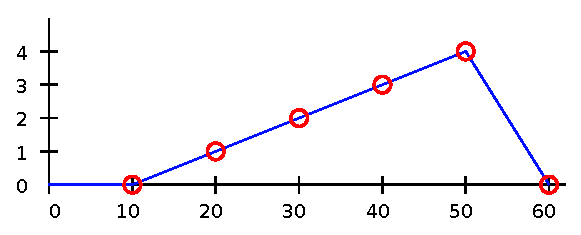
\includegraphics[width=\textwidth]{imatges/rrdtool/mostreig_regular.eps}
  \caption{Moviment d'un mòbil: perfil de velocitat en blau, punts de mostreig en vermell}
  \label{fig:rrdtool:mostreig_regular}
\end{figure}

En primer lloc, es crea una base de dades de nom \emph{velocitat.rrd} amb un temps de mostreig de 10 segons i un registre anomenat \emph{mps} que emmagatzema la velocitat del mòbil.
\begin{lstlisting}[style=sh]
export TZ=UTC
rrdtool create velocitat.rrd --start 1262304000 --step 10 \
        DS:mps:GAUGE:600:-U:U                              \ 
        RRA:AVERAGE:0.5:1:24                                                   
\end{lstlisting}


En segon lloc, s'actualitza la base de dades amb els valors $x=[0,1,2,3,4,0]$ que s'han mesurat als temps $t=[10,20,30,40,50,60]$.
\begin{lstlisting}[style=sh]
rrdtool update velocitat.rrd 1262304010:0 1262304020:1 1262304030:2 1262304040:3 1262304050:4 1262304060:0
\end{lstlisting}

Si es mostra el contingut de la base de dades, amb \verb+rrdtool dump+, es pot veure com els valors han entrat correctament:
\begin{lstlisting}
00:00:00 UTC  --> <row><v>NaN</v></row>
00:00:10 UTC  --> <row><v>0.0000000000e+00</v></row>
00:00:20 UTC  --> <row><v>1.0000000000e+00</v></row>
00:00:30 UTC  --> <row><v>2.0000000000e+00</v></row>
00:00:40 UTC  --> <row><v>3.0000000000e+00</v></row>
00:00:50 UTC  --> <row><v>4.0000000000e+00</v></row>
00:01:00 UTC  --> <row><v>0.0000000000e+00</v></row>
\end{lstlisting}


Finalment, es demana a RRDtool que faci un gràfic dels valors anteriors, el resultat es pot veure a la figura~\ref{fig:rrdtool:velocitat}:
\begin{lstlisting}[style=sh]
rrdtool graph velocitat.eps -a EPS --start 1262303999 --end 1262304060 DEF:vel=velocitat.rrd:mps:AVERAGE LINE1:vel#0000FF:"velocitat en m/s\l" -v "m/s" --x-grid SECOND:10:SECOND:10:SECOND:10:0:%X
\end{lstlisting}

\begin{figure}[htp]
  \centering
  \includegraphics[width=\textwidth]{imatges/rrdtool/velocitat.eps}
  \caption{Velocitats emmagatzemades a RRDtool d'un tipus Gauge}
  \label{fig:rrdtool:velocitat}
\end{figure}



D'aquest gràfic es desprèn com RRDtool interpreta les sèries temporals en sentit de passat. Els valors desats es representen constants en l'interval anterior al temps que els correspon. En l'exemple, a l'interval de temps (0,10] hi ha el valor 0, en l'interval (10,20] hi ha el valor 2, etc. En el temps 0, el valor és desconegut ja que no hi ha informació per l'interval anterior a zero.

Concloent, aquest és un exemple mostrejat de manera poc adequada  segons la idea de RRDtool. El mòbil de la figura~\ref{fig:rrdtool:mostreig_regular} té un perfil de velocitats mostrejat amb el valor instantani i aquest correspondria al mateix cas que mesurar una magnitud com la temperatura. Per mostrejar amb la idea de velocitat de RRDtool caldria que la velocitat fos constant; de fet, aleshores el perfil de velocitats original seria el de la figura~\ref{fig:rrdtool:velocitat}.

Si la velocitat no és constant, com és el cas de l'exemple, aleshores per complir amb la idea de RRDtool el valor mostrejat hauria d'informar de la velocitat en el darrer interval. Per exemple, amb la velocitat mitjana de cada interval ($x=[0,\ 0{,}5,\ 1{,}5,\ 2{,}5,\ 3{,}5 ,\ 2]$) ja s'aconsegueix una millor aproximació a la idea de RRDtool. Encara és més, en el concepte de RRDtool aquest exemple s'hauria de passar al domini de comptadors; és a dir mesurar l'espai recorregut en comptes de la velocitat. En els apartats següents es tractarà amb més detall els comptadors.


\subsection{Comptador monòton: \emph{Counter}}

Les dades de tipus Counter són dades provinents de comptadors. Aquestes dades no són velocitats i per tant cal aplicar transformació. 

Un comptador és un aparell de mesura que comença a zero i es va incrementant de manera contínua i monòtona en relació al paràmetre que està mesurant. A diferència d'una magnitud, un comptador no només indica el valor instantani de la variable sinó que informa dels valors des de l'última mesura. En anglès hi ha dues paraules que es tradueixen com a comptador: \emph{counter}, utilitzat en general, i \emph{meter}, utilitzat per exemple en energia elèctrica, en gas, en odometria, etc.

Per a transformar els valors d'un comptador a velocitat, a RRDtool se segueix el procediment següent.
En un moment determinat es pren el valor del comptador i al cap d'un temps definit es torna a consultar. Fent la diferència dels dos valors s'obté l'increment. Si a més es divideix per la diferència dels temps, el resultat és la mitjana del valor per unitat de temps; és a dir, una velocitat. A RRDtool el temps es mesura en segons, per tant les velocitats sempre es desen amb unitats de \emph{magnitud/s}. 
\begin{equation}\label{eq:rrdtool:rate}
c_2 \geq c_1 \longrightarrow\text{mitjana per }u.t. =\frac{c_2-c_1}{t_2-t_1}
\end{equation}
on $c_2$ i $t_2$ són el valor del comptador i el temps actual  i $c_1$ i $t_1$ són en el temps anterior.

RRDtool només emmagatzema velocitats. Per tant en les dades tipus comptador sempre calcula aquesta proporció mitjana del valor en cada període. Per exemple si el comptador mesura quilòmetres (km), el valor desat són velocitats (km/s).
Per aquesta mateixa raó, el primer valor que es desa a la base de dades no es pot calcular, ja que l'anterior no existeix, i es considera desconegut.

Els comptadors no poden decréixer però tenen un valor màxim que quan hi arriben tornen a començar des de zero. És a dir, els comptadors es poden desbordar (\emph{counter wraps}). RRDtool té en compte aquest cas i calcula l'increment real que s'ha produït. 
\begin{equation}\label{eq:rrdtool:wrap}
c_2 < c_1 \longrightarrow \text{mitjana per }u.t. =\frac{(\text{fons d'escala} -c_1)+c_2}{t_2-t_1}
\end{equation}
on ara, a diferència de l'equació~\ref{eq:rrdtool:rate}, cal tenir en compte el fons d'escala del comptador. 

Ara bé, de moment RRDtool només reconeix comptadors de 32 o 64 bits, els quals tenen rangs hexadecimals de 0 a FFFFFFFF$_h$ i de 0 a FFFFFFFFFFFFFFFF$_h$ respectivament. Si el rang del comptador és diferent d'aquests dos, el valor calculat és erroni
\footnote{En comptes del tipus \emph{counter} es pot utilitzar el tipus \emph{derive} amb el límit de velocitat mínima a zero. Llavors no es calculen valors erronis en els desbordaments sinó que es consideren desconeguts. Sigui quina sigui la manera, RRDtool no sap tractar aquests comptadors de manera adequada.\label{peu:rrdtool:counter}}.

Alguns exemples de comptador són el comptaquilòmetres d'un cotxe, els bytes transferits d'un router, la quantitat de pàgines impreses, el nombre de visitants, etc.


\paragraph{Exemple} Ara en el mòbil anterior de la figura~\ref{fig:rrdtool:velocitat}, en comptes de mesurar la velocitat es mesura l'espai recorregut com es veu a la figura~\ref{fig:rrdtool:mostreig_comptador}, també cada 10 segons. 

\begin{figure}[htp]
  \centering
  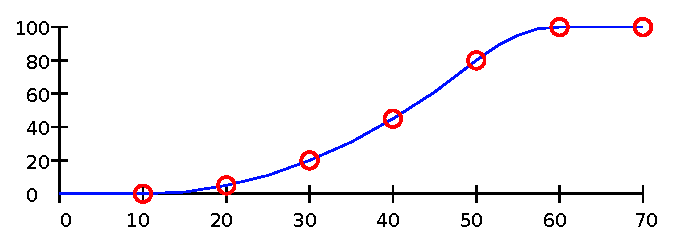
\includegraphics[width=\textwidth]{imatges/rrdtool/mostreig_comptador.eps}
  \caption{Moviment d'un mòbil: perfil d'espai recorregut en blau, punts de mesura en vermell}
  \label{fig:rrdtool:mostreig_comptador}
\end{figure}

En primer lloc, es crea una base de dades de nom \emph{comptador.rrd} amb un temps de mostreig de 10 segons i un registre anomenat \emph{mps} que emmagatzema la velocitat del mòbil però les dades d'entrada són l'espai recorregut.
\begin{lstlisting}[style=sh]
export TZ=UTC
rrdtool create comptador.rrd --start 1262304000 --step 10 \
        DS:mps:COUNTER:600:-U:U                           \ 
        RRA:AVERAGE:0.5:1:24                                                   
\end{lstlisting}

En segon lloc, s'actualitza la base de dades amb els valors $x=[0,5,20,45,80,100,100]$ que s'han mesurat als temps $t=[10,20,30,40,50,60,70]$ 

\begin{lstlisting}[style=sh]
rrdtool update comptador.rrd 1262304010:0 1262304020:5 1262304030:20 1262304040:45 1262304050:80 1262304060:100 1262304070:100
\end{lstlisting}

Si es mostra el contingut de la base de dades es pot veure com no hi ha els mateixos valors que s'han inserit; 
el gràfic de la figura~\ref{fig:rrdtool:comptador} que ha generat  RRDtool també corrobora aquestes dades:
\begin{lstlisting}
00:00:00 UTC  --> <row><v>NaN</v></row>
00:00:10 UTC  --> <row><v>NaN</v></row>
00:00:20 UTC  --> <row><v>5.0000000000e-01</v></row>
00:00:30 UTC  --> <row><v>1.5000000000e+00</v></row>
00:00:40 UTC  --> <row><v>2.5000000000e+00</v></row>
00:00:50 UTC  --> <row><v>3.5000000000e+00</v></row>
00:01:00 UTC  --> <row><v>2.0000000000e+00</v></row>
00:01:10 UTC  --> <row><v>0.0000000000e+00</v></row>
\end{lstlisting}

 
\begin{figure}[htp]
  \centering
  \includegraphics[width=\textwidth]{imatges/rrdtool/comptador.eps}
  \caption{Velocitats emmagatzemades a RRDtool d'un tipus Counter}
  \label{fig:rrdtool:comptador}
\end{figure}

En aquest gràfic, on les unitats són de metres per segon, es veu l'efecte de desar les dades en velocitat. Com que l'entrada de dades és de tipus comptador, RRDtool s'encarrega de transformar els valor a velocitat segons les equacions \ref{eq:rrdtool:rate} i \ref{eq:rrdtool:wrap} i també es compleix que el primer valor inserit s'emmagatzema com a desconegut ja que no es pot calcular. 

En referència a l'espai recorregut, es pot calcular multiplicant cada valor emmagatzemat pel temps de mostreig (10 segons). Aleshores s'obté 
$[u , 5 , 15 , 25 , 35 , 20 , 0]$
a on cada valor és l'increment d'espai recorregut en cada interval de temps corresponent; és a dir en els intervals
$[\ (0,10], (10,20], \ldots, (60,70]\ ]$.
 Per calcular l'espai recorregut total entre el temps 10 i el temps 70 s'ha de sumar aquests increments, aleshores s'obté el comptatge total de 100 metres que es correspon correctament amb el de la figura~\ref{fig:rrdtool:mostreig_comptador}.





\subsection{Comptador doble:  \emph{Derive}}

Les dades de tipus derive són de tipus comptador que tant pot incrementar com decrementar el valor; per això l'anomenem comptador doble. Aquestes dades no són velocitats i per tant cal aplicar transformació. 

La transformació a velocitat es calcula amb l'equació~\ref{eq:rrdtool:rate}, de la mateixa manera que els comptadors de tipus \emph{counter}. Però en els \emph{derive} no es té en compte el desbordament, sinó que un decrement del comptador es transforma a una velocitat negativa:  
$$
\text{mitjana per }u.t. =\frac{c_2-c_1}{t_2-t_1}
$$

Com que es desactiva el detector de desbordaments, el tipus \emph{derive} també s'utilitza per als \emph{counter} que no són ni de 32 ni de 64 bits. En aquests casos es configura el límit mínim de velocitat a zero i quan hi ha el desbordament\footnote{Això no es pot considerar una bona solució, vegeu nota~\ref{peu:rrdtool:counter}.} el valor transformat es considera desconegut, ja que la velocitat calculada és inferior al límit imposat de valor zero. 

Alguns exemples de comptador \emph{derive} són una bomba de cabal que pot bombejar o succionar, un comptador elèctric que mesura el total d'energia consumida menys la produïda, el balanç de població que emigra menys la que immigra, el saldo d'una llibreta que té ingressos i despeses, la quantitat de productes d'una màquina de \emph{vending}, etc. 


\paragraph{Exemple} Es mesura el saldo d'una llibreta d'estalvi que inicialment està a 0\euro, al cap de 10 segons rep un ingrés de 10\euro, al cap de 10 segons rep 20\euro\ i al cap de 10 segons té una despesa de 15\euro. 

Els valors que va prenent la llibreta (el comptador) es poden veure a la figura~\ref{fig:rrdtool:mostreig_derive}. Les mostres es prenen a l'instant abans que es faci l'operació d'ingrés o despesa; és a dir que la llibreta mostra el valor que ha tingut a l'interval anterior, la qual és la manera com s'entenen les sèries temporals a RRDtool. 

\begin{figure}[htp]
  \centering
  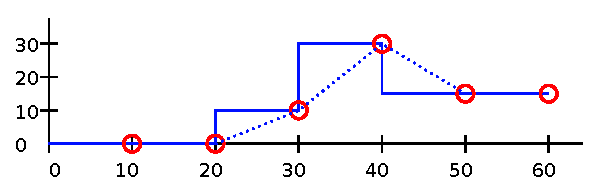
\includegraphics[width=\textwidth]{imatges/rrdtool/mostreig_derive.eps}
  \caption{Llibreta d'estalvi: valor del saldo en blau, punts de mesura en vermell}
  \label{fig:rrdtool:mostreig_derive}
\end{figure}

A més, RRDtool entén que les variables mesurades són contínues. Per tant amb les mesures fetes de la llibreta entén que el valor s'ha incrementat de manera contínua en tot l'interval. Això es pot observar a la línia discontínua de la figura~\ref{fig:rrdtool:mostreig_derive}, que és l'aproximació que fa RRDtool ja que només es guarda la velocitat mitjana a l'interval.

Es crea una base de dades de nom \emph{derive.rrd} amb un temps de mostreig de 10 segons i un registre anomenat \emph{eurps} que emmagatzema la velocitat del comptador (del saldo de la llibreta) a partir de les lectures del saldo. 

\begin{lstlisting}[style=sh]
export TZ=UTC
rrdtool create derive.rrd --start 1262304000 --step 10 \
        DS:eurps:DERIVE:600:-U:U                       \ 
        RRA:AVERAGE:0.5:1:24                                                   
\end{lstlisting}


S'actualitza la base de dades amb els valors $x=[0,0,10,30,15,15]$ que s'han mesurat als temps $t=[10,20,30,40,50,60]$ 

\begin{lstlisting}[style=sh]
rrdtool update derive.rrd 1262304010:0 1262304020:0 1262304030:10 1262304040:30 1262304050:15 1262304060:15
\end{lstlisting}

A continuació es mostren els valors emmagatzemats i a la figura~\ref{fig:rrdtool:derive} es mostra el gràfic que genera RRDtool:
\begin{lstlisting}
00:00:00 UTC  --> <row><v>NaN</v></row>
00:00:10 UTC  --> <row><v>NaN</v></row>
00:00:20 UTC  --> <row><v>0.0000000000e+00</v></row>
00:00:30 UTC  --> <row><v>1.0000000000e+00</v></row>
00:00:40 UTC  --> <row><v>2.0000000000e+00</v></row>
00:00:50 UTC  --> <row><v>-1.5000000000e+00</v></row>
00:01:00 UTC  --> <row><v>0.0000000000e+00</v></row>
\end{lstlisting}


\begin{figure}[htp]
  \centering
  \includegraphics[width=\textwidth]{imatges/rrdtool/derive.eps}
  \caption{Velocitats emmagatzemades a RRDtool d'un tipus Derive}
  \label{fig:rrdtool:derive}
\end{figure}

Aquest gràfic és com l'analitzat en l'exemple dels tipus \emph{counter} (figura~\ref{fig:rrdtool:comptador}), amb la diferència que ara en els \emph{derive} hi apareixen velocitats negatives. 
Com s'ha fet en els \emph{counter}, es pot calcular els increments de saldo de cada interval multiplicant les velocitats pel temps de mostreig. Aleshores els increments de saldo són $[u,0,10,20,-15,0]$ que sumats donen correctament els 15\euro\ de saldo final de la figura~\ref{fig:rrdtool:mostreig_derive}.


\subsection{Comptador relatiu: \emph{Absolute}}

Les dades de tipus Absolute són de tipus comptador d'increments; per això l'anomenen comptador relatiu. Aquestes dades no són velocitats i per tant cal aplicar transformació. 

Un comptador d'increments mesura directament la diferència des de l'última lectura, es pot veure com un comptador que es posa a zero a cada lectura. Per tant, per transformar les mesures a velocitat es divideix l'increment per la diferència de temps
$$
\text{mitjana per }u.t. =\frac{\Delta c}{t_2-t_1}
$$
on ara, a diferència de l'equació~\ref{eq:rrdtool:rate}, es mesura directament el comptatge ($\Delta c$) des de la mesura anterior.

Els increments mesurats poden ser positius o negatius; és a dir com en el cas \emph{derive} les velocitats resultants poden ser positives o negatives. Per tant, el tipus \emph{absolute} és el mateix que el \emph{derive} amb la diferència que el valor mesurat, el qual és el valor actual del comptador,  és un increment.

El primer valor que es desa a la base de dades ara es pot calcular, a diferència dels comptadors \emph{counter} i \emph{derive}. En aquest dos cal calcular l'increment de comptatge i en el primer valor és desconegut, ja que podria ser erroni suposar-lo com a zero. En el cas del comptador \emph{absolute} també cal indicar quin és el temps inicial, però aquest es considera que és el mateix que el d'inici de la base de dades.

Alguns exemples de comptador \emph{absolute} són els mateixos que en el \emph{derive} però mesurats de manera relativa: increments de bombeig o succió d'una bomba, la mesura de l'energia elèctrica en un cert temps, els increments de població degut a la migració, els registres a una llibreta, la venda o repostatge de productes, etc.

\paragraph{Exemple} Com en l'exemple del tipus \emph{derive} (figura~\ref{fig:rrdtool:mostreig_derive}), es mesura el saldo d'una llibreta d'estalvi. Ara, però, les mesures de comptador són les operacions d'ingrés o de despesa. El saldo pren els mateixos valors que en l'exemple anterior però ara les mesures són els increments, positius o negatius, que es poden veure a la figura~\ref{fig:rrdtool:mostreig_absolute}. 

\begin{figure}[htp]
  \centering
  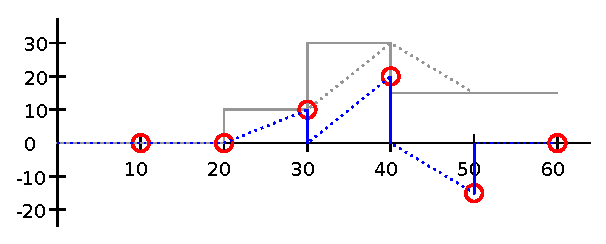
\includegraphics[width=\textwidth]{imatges/rrdtool/mostreig_absolute.eps}
  \caption{Llibreta d'estalvi: increments de saldo en blau, punts de mesura en vermell, saldo en gris}
  \label{fig:rrdtool:mostreig_absolute}
\end{figure}

Les línies discontínues segueixen mostrant, com a la figura~\ref{fig:rrdtool:mostreig_derive}, l'aproximació que RRDtool fa del comptador com a variable contínua. 


Es crea una base de dades de nom \emph{absolute.rrd} amb un temps de mostreig de 10 segons i un registre anomenat \emph{eurps} que emmagatzema la velocitat del comptador (el saldo de la llibreta) a partir dels increments de saldo. 
\begin{lstlisting}[style=sh]
export TZ=UTC
rrdtool create absolute.rrd --start 1262304000 --step 10 \
        DS:eurps:ABSOLUTE:600:-U:U                        \ 
        RRA:AVERAGE:0.5:1:24                                                   
\end{lstlisting}


S'actualitza la base de dades amb els valors $x=[0,0,10,20,-15,0]$ que s'han mesurat als temps $t=[10,20,30,40,50,60]$ 
\begin{lstlisting}[style=sh]
rrdtool update absolute.rrd 1262304010:0 1262304020:0 1262304030:10 1262304040:20 1262304050:-15 1262304060:0
\end{lstlisting}

A continuació es mostren els valors emmagatzemats i a la figura~\ref{fig:rrdtool:absolute} es mostra el gràfic que genera RRDtool; és idèntic a la figura~\ref{fig:rrdtool:derive} però ara el primer valor és conegut.:
\begin{lstlisting}
00:00:00 UTC  --> <row><v>NaN</v></row>
00:00:10 UTC  --> <row><v>0.0000000000e+00</v></row>
00:00:20 UTC  --> <row><v>0.0000000000e+00</v></row>
00:00:30 UTC  --> <row><v>1.0000000000e+00</v></row>
00:00:40 UTC  --> <row><v>2.0000000000e+00</v></row>
00:00:50 UTC  --> <row><v>-1.5000000000e+00</v></row>
00:01:00 UTC  --> <row><v>0.0000000000e+00</v></row>
\end{lstlisting}


\begin{figure}[htp]
  \centering
  \includegraphics[width=\textwidth]{imatges/rrdtool/absolute.eps}
  \caption{Velocitats emmagatzemades a RRDtool d'un tipus Absolute}
  \label{fig:rrdtool:absolute}
\end{figure}

D'aquest gràfic, com en el casos \emph{derive} i \emph{counter}, es pot obtenir els increments de comptatge a cada interval si es multiplica cada valor pel temps de mostreig (10 segons). Aquests valors es podrien observar en un gràfic de barres, tot i que RRDtool només treballa amb variables velocitat contínues i per tant no pot mostrar exactament aquest gràfics de barres del comptador. A la figura~\ref{fig:rrdtool:comptador_barres} s'utilitza RRDtool perquè dibuixi els valors pintant l'àrea i multiplicant l'escala de l'eix Y per 10; perquè fos un gràfic de barres cal imaginar que a l'eix X hi ha les etiquetes corresponents als intervals: $(0,10], (10,20], \ldots, (50,60]$ i que cada un d'aquest intervals és una barra.

\begin{figure}[htp]
  \centering
  \includegraphics[width=\textwidth]{imatges/rrdtool/comptador_barres.eps}
  \caption{Gràfic de barres a RRDtool d'un comptador}
  \label{fig:rrdtool:comptador_barres}
\end{figure}

Ara bé, RRDtool sí que té funcions per tractar amb càlculs típics dels comptadors, per exemple calcular el total del comptador en un interval de temps donat. En aquest cas, el total del comptador des de l'inici fins a una data correspon al saldo de la llibreta en aquella data. A continuació es calcula el saldo des del temps 0 fins al temps 60, el qual correspon als 15\euro\ de la figura~\ref{fig:rrdtool:mostreig_absolute}.:
\begin{lstlisting}[style=sh]
rrdtool graphv absolute.eps -a EPS --start 1262303999 --end 1262304060 DEF:saldo=absolute.rrd:eurps:AVERAGE VDEF:tot=saldo,TOTAL PRINT:tot:%lf\EUR/s
\end{lstlisting}

\begin{lstlisting}
print[0] = "15.000000EUR/s"
\end{lstlisting}

\section[Normalització]{Normalització de l'interval}
\label{sec:rrdtool-etapes:normalitzacio}

RRDtool emmagatzema les dades a intervals regulars, és a dir en el temps de mostreig desitjat (anomenat \emph{step}). Com que a la pràctica és difícil complir-lo amb exactitud, cal modificar les dades perquè encaixin en aquest temps; és a dir s'ha de normalitzar l'interval de la sèrie temporal.

Per a modificar els valors de la sèrie temporal, en el context de velocitat vist a l'apartat anterior es pot plantejar una modificació de dades que tracti de mantenir l'àrea de sota la corba. La interpretació física és que es manté la quantitat total de magnitud.
Per exemple si les dades són velocitats lineals en m/s es pot entendre el problema com que es modifica la velocitat però es manté l'espai recorregut. O bé si les dades són comptadors, com que s'ha desat la velocitat s'entén que s'està mantenint la quantitat total.

Així doncs, el problema a resoldre és el següent. Donada una sèrie temporal acotada a un temps final $T_F$
$$%
S=\{\mathbf{X(t)}; t=t_0,t_1,t_2,\ldots,t_F\}
$$
que no té un període de mesura regular 
$$
t_{i+1}\neq t_{i} + T 
$$
es vol convertir a una sèrie temporal normalitzada amb interval regulars tal que ara $T$ correspongui al període de mostreig $t_m$:
$$%
S^N=\{\mathbf{X^N(t^N)}; t^N=t_0,t_1,t_2,\ldots,t_k\}
$$
$$
t^N_{k+1}= t^N_{k} + t_m 
$$
$$
t^N_k < T_F
$$
on $N$ indica que els valors i els temps ara contenen els valors normalitzats:
$$
\mathbf{X^N}= [x^N(t^N_0),x^N(t^N_1),\ldots,x^N(t^N_{T_i})]
$$

En resum, el vector de mesures té la forma 
$$
\mathbf{X(t)} = [x_0,x_1,\ldots,x_{F-1},x_F]
$$
i amb la mateixa mida el vector de temps de mesures
$$
\mathbf{t}=[t_0,t_1 \ldots, t_{T_f-1}, t_{T_f} ]
$$

Però el vector de valors normalitzats té una mida diferent 
$$
\mathbf{X^N(t^N)} = [x^N_0, x^N_1, \ldots,x^N_k ]
$$
on el vector de temps de mostreig normalitzats té la forma
$$
\mathbf{t^N}=[0,t_m, 2t_m,3t_m, \ldots kt_m ]
$$


A l'hora de convertir la sèrie temporal RRDtool utilitza el criteri de mantenir constant l'àrea sota la corba; a l'apartat~\ref{sec:rrdtool-etapes:gauge} s'ha vist com RRDtool representa les sèries temporals en velocitat i en passat. En els exemples d'aquest apartat, però, les mesures es feien en el temps de mostreig exacte, a continuació es mostrarà com RRDtool gestiona els casos en els que les mostres no coincideixen amb el temps de mostreig.

\subsection{Mostreig en temps real}

En un primer cas, la sèrie temporal original està mostrejada amb un únic valor a cada interval, tal com es faria en un sistema en temps real 
$$
\mathbf{X(t)}= [x(t_0)\ldots,x(t_{T_f-1}),x(t_{T_f})]
$$
$$
0< t_0 < t^N_1 < \cdots <   t^N_{i-1}<t_{T_f-1} < t^N_i < t_{T_f}
$$ 

En aquest cas, la sèrie temporal no té intervals regulars però sí que hi ha garantits uns terminis temporals en els que es disposa d'un valor i només hi ha un valor a cada interval:
$$
t_{i+1}\neq t_{i} + T 
$$
$$
t_{i+1} - t_{i} \leq t_m 
$$

A continuació es detalla com RRDtool normalitza la sèrie temporal en l'interval $[t^N_{i-1},t^N_i]$, es pot veure una interpretació gràfica a la figura~\ref{fig:rrdtool:normalitzacio}.

\begin{figure}[htp]
  \centering
  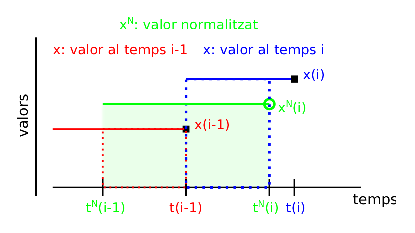
\includegraphics[width=\textwidth]{imatges/rrdtool/normalitzacio.eps}
  \caption{Normalització d'un interval}
  \label{fig:rrdtool:normalitzacio}
\end{figure}


Per una banda, es calcula l'àrea en l'interval seleccionat a partir dels valors mesurats
\[
A([t^N_{i-1},t^N_i]) = A([t^N_{i-1},t_{i-1}])+A([t_{i-1},t^N_i]) = ( t_{i-1} - t^N_{i-1})x_{i-1} + ( t^N_{i} - t_{i-1} )x_{i}
\]
i per altra banda, la normalització de l'interval s'expressa amb un valor de velocitat $X^N_i$ que es representa en el temps  $t^N_i$ degut a que RRDtool interpreta els valors en passat (constants en l'interval anterior)
\[
A^N = (  t^N_i - t^N_{i-1} )x^N_i  = t_m x^N_i
\]
Aleshores, s'igualen les dues expressions per tal que en normalitzar es conservi l'àrea en l'interval
\[
A^N=A([t^N_{i-1},t^N_i])
\]
d'on aïllant s'obté l'equació del valor normalitzat 
\begin{equation}\label{eq:rrdtool-etapes:normalitza}
x^N_i= \frac{(t_{i-1}-t^N_{i-1})x_{i-1} + (t^N_i-t_{i-1})x_i  }{t_m}
\end{equation}


El mateix es pot aplicar per tots els intervals de $\mathbf{X}$ per obtenir $\mathbf{X^N}$.



\paragraph{Exemple}


Agafem una nova base de dades velocitat.rrd i ara l'actualitzem amb el mateix perfil de velocitat de la figura~\ref{fig:rrdtool:mostreig_regular} però mostrejat de manera irregular com es veu a la figura~\ref{fig:rrdtool:mostreig_irregular}. A cada interval de mostreig hi segueix havent una mesura, i per tant compleixen el període de mostreig, però el temps de mostreig és irregular. Així ara els valors de velocitat mesurats són $x=[0, 0{,}5 , 1 , 2{,}8 , 3{,}2 , 2 , 0]$ en els temps $t=[10,15,20,38,42,55,65]$.


\begin{figure}[htp]
  \centering
  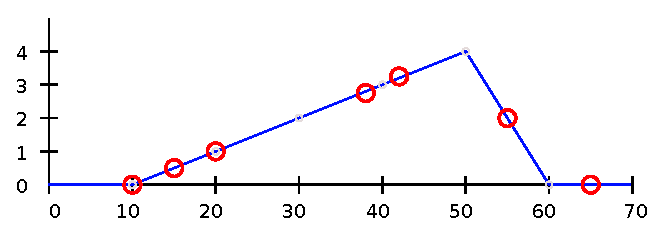
\includegraphics[width=\textwidth]{imatges/rrdtool/mostreig_irregular.eps}
  \caption{Mostreig en temps real: perfil de velocitat en blau, punts de mesura irregulars en vermell, període de mostreig de 10 segons}
  \label{fig:rrdtool:mostreig_irregular}
\end{figure}

S'insereixen els valors a la base de dades:
\begin{lstlisting}[style=sh]
rrdtool update velocitat.rrd 1262304010:0 1262304015:0.5 1262304020:1 1262304038:2.8 1262304042:3.2 1262304055:2 1262304065:0
\end{lstlisting}

A continuació es mostren els valors emmagatzemats i el gràfic que genera RRDtool (figura~\ref{fig:rrdtool:velocitat_irregular}):
\begin{lstlisting}
00:00:00 UTC  --> <row><v>NaN</v></row>
00:00:10 UTC  --> <row><v>0.0000000000e+00</v></row>
00:00:20 UTC  --> <row><v>7.5000000000e-01</v></row>
00:00:30 UTC  --> <row><v>2.8000000000e+00</v></row>
00:00:40 UTC  --> <row><v>2.8800000000e+00</v></row>
00:00:50 UTC  --> <row><v>2.2400000000e+00</v></row>
00:01:00 UTC  --> <row><v>1.0000000000e+00</v></row>
\end{lstlisting}


\begin{figure}[htp]
  \centering
  \includegraphics[width=\textwidth]{imatges/rrdtool/velocitat_irregular.eps}
  \caption{Valors emmagatzemats a RRDtool d'un mostreig en temps real}
  \label{fig:rrdtool:velocitat_irregular}
\end{figure}

Aplicant l'equació~\ref{eq:rrdtool-etapes:normalitza} als valors mesurats es pot comprovar que s'obtenen els valors normalitzats calculats per RRDtool 
$\mathbf{X^N}=[u , 0 , 0{,}75 , 2{,}8 , 2{,}88 , 2{,}24 , 1]$. 
Cal notar que a RRDtool el primer valor normalitzat, el qual correspon al temps $t^N_0$, és desconegut ja que no s'admeten insercions en el temps $t_0$.


\subsection{Ultramostreig}

En la normalització anterior de mostreig en temps real, en cada període de mostreig només hi havia una mesura. Ara bé, RRDtool permet que en cada interval hi hagi més d'una mesura i per tant hi pot haver més d'un valor a l'hora de normalitzar; anomenem aquest mostreig com ultramostreig (\emph{upsampling}), representat a la figura~\ref{fig:rrdtool-etapes:ultramostreig}.
$$
\mathbf{X(t)}= [x(t_0)\ldots,x(t_{T_f-k}),\cdots,x(t_{T_f-2}),x(t_{T_f-1}),x(t_{T_f})]
$$
$$
0< t_0 < t^N_1 < \cdots <   t^N_{i-1}<t_{T_f-k} <\cdots< t_{T_f-1} < t^N_i < t_{T_f}
$$

\begin{figure}[tbp]
  \centering
  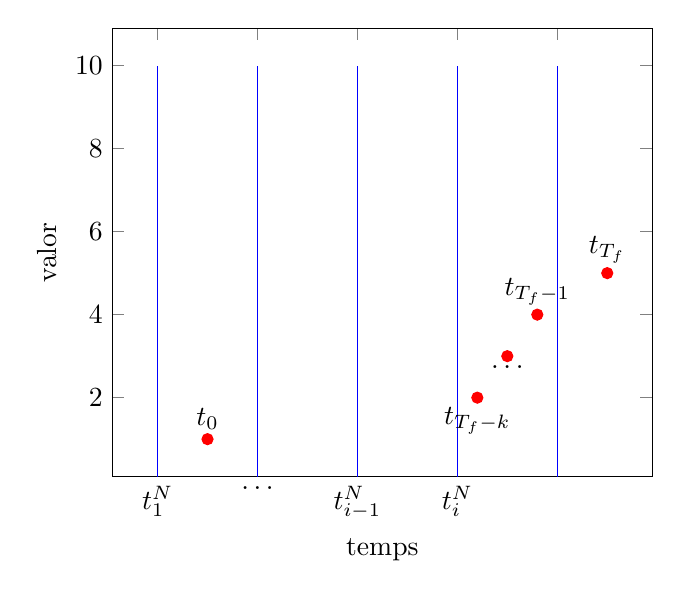
\begin{tikzpicture}
    \begin{axis}[
        xlabel=temps ,
        ylabel= valor,
        xticklabels={0,$t_1^N$,$\ldots$,$t_{i-1}^N$,$t_i^N$},
        ]
    \addplot[ycomb,blue] coordinates {
        (0,10)
        (10,10)
        (20,10)
        (30,10)
        (40,10)
    }; 
 
    \addplot[only marks,mark=*,red] coordinates {
        (5,1)
        (32,2)
        (35,3)
        (38,4)
        (45,5)
    };

    \node[above] at (axis cs:5,1) {$t_0$};
    \node[below] at (axis cs:32,2) {$t_{T_f -k}$};
    \node[below] at (axis cs:35,3) {$\ldots$};
    \node[above] at (axis cs:38,4) {$t_{T_f -1}$};
    \node[above] at (axis cs:45,5) {$t_{T_f}$};

    \end{axis}
  \end{tikzpicture}
  \caption{Representació d'ultramostreig}
  \label{fig:rrdtool-etapes:ultramostreig}
\end{figure}

Aleshores, el valor normalitzat es calcula de la mateixa manera que a l'equació~\ref{eq:rrdtool-etapes:normalitza}, però ara el càlcul és una ponderació pel temps de tots els valors que cauen a dins de l'interval de normalització
\begin{equation}\label{eq:rrdtool:ultramostreig}
x^N_i = \frac{ (t_{T_f-k}-t^N_{i-1})x_{f-k} + \cdots + (t_{T_f-1}-t_{T_f-2})x_{f-1} + (t^N_i-t_{T_f-1})x_f }{t_m}
\end{equation}


Seguint aquesta equació de manera iterativa, es pot calcular el vector de valors normalitzats $\mathbf{X^N}$  per tots els $\mathbf{X(t)}$ amb l'algoritme següent:

\begin{lstlisting}[mathescape=true]  
Normalització d'una sèrie temporal amb ultramostreig 
a períodes de mostreig regulars 
INPUT: 
      vector de valors $\mathbf{X} = [x_0,x_1,\ldots,x_f]$ 
      vector de temps $\mathbf{t} = [t_0,t_1,\ldots,t_f]$
      període de mostreig regular  $t_m$
OUTPUT: 
      vector de valors normalitzats $\mathbf{X^N} = [x_0^N,x_1^N,\ldots,x_k^N]$

$x^N_0$ := unknown
$t^N_0$ := 0
$t^N_1$ := $t_0^N$ + $t_m$
i := 1

$A$ := $x_0t_0$   <-- àrea acumulada inicial 
k := 1

mentre k $\leq$ dim(x) fes

    si $t_k < t_i^N$ llavors
        $A$ := $A + x_k( t_k-t_{k-1}) $ <-- acumulació
        k := k+1
    sino 
        $x_i^N$ := $\dfrac{A + x_k( t_i^N-t_{k-1} )}{t_m}$

        $t_{i+1}^N$ := $t_i^N$ + $t_m$
        $A$ := $x_k*( t_k-t_i^N )$ <-- àrea acumulada inicial 
        k := k+1
        i := i+1
    fsi 

fmentre

\end{lstlisting}

\paragraph{Exemple}

Agafem una nova base de dades velocitat.rrd i ara l'actualitzem amb el mateix perfil de velocitat de la figura~\ref{fig:rrdtool:mostreig_regular} però amb més mostres en algun interval com es veu a la figura~\ref{fig:rrdtool:ultramostreig}. A cada interval de mostreig hi segueix havent com a mínim una mesura i compleixen el període de mostreig però en algun interval hi ha més d'una mostra. Així ara el valors de velocitat mesurats són $x=[0 , 0{,}5 , 0{,}8 , 1 , 2{,}8 , 3{,}2 , 3{,}5 , 3{,}8 , 2 , 0]$ en els temps $t=[10 , 15 , 18, 20, 38, 42, 45, 48, 55, 65]$.


\begin{figure}[htp]
  \centering
  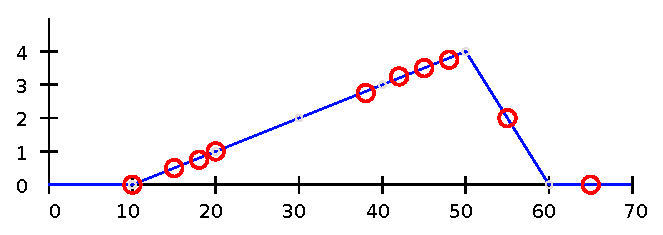
\includegraphics[width=\textwidth]{imatges/rrdtool/sobremostreig.eps}
  \caption{Ultramostreig: perfil de velocitat en blau, punts de mesura (alguns ultramostrejats) en vermell, període de mostreig de 10 segons}
  \label{fig:rrdtool:ultramostreig}
\end{figure}

S'insereixen els valors a la base de dades:
\begin{lstlisting}[style=sh]
rrdtool update velocitat.rrd 1262304010:0 1262304015:0.5 1262304018:0.8 1262304020:1 1262304038:2.8 1262304042:3.2 1262304045:3.5 1262304048:3.8 1262304055:2 1262304065:0
\end{lstlisting}

A continuació es mostren els valors emmagatzemats i el gràfic que genera RRDtool (figura~\ref{fig:rrdtool:velocitat_ultramostrejada}):

\begin{lstlisting}
00:00:00 UTC  --> <row><v>NaN</v></row>
00:00:10 UTC  --> <row><v>0.0000000000e+00</v></row>
00:00:20 UTC  --> <row><v>6.9000000000e-01</v></row>
00:00:30 UTC  --> <row><v>2.8000000000e+00</v></row>
00:00:40 UTC  --> <row><v>2.8800000000e+00</v></row>
00:00:50 UTC  --> <row><v>3.2300000000e+00</v></row>
00:01:00 UTC  --> <row><v>1.0000000000e+00</v></row>
\end{lstlisting}


\begin{figure}[htp]
  \centering
  \includegraphics[width=\textwidth]{imatges/rrdtool/velocitat_sobremostrejada.eps}
  \caption{Valors emmagatzemats a RRDtool d'un ultramostreig}
  \label{fig:rrdtool:velocitat_ultramostrejada}
\end{figure}

Respecte a la figura~\ref{fig:rrdtool:velocitat_irregular} del cas de mostreig en temps real, ara només han canviat els valors dels intervals ultramostrejats mentre que els altres intervals continuen valent el mateix: $\mathbf{X^N}=[u , 0 , \underline{0{,}69} , 2{,}8 , 2{,}88 , \underline{2{,}24} , 1]$. Els valors que canvien són molt semblants als anteriors, però es pot dir que es té una millor aproximació a la velocitat real ja que en aquests intervals s'ha mostrejat més.

\subsection{Inframostreig}

Per altra banda, quan en un interval no hi ha cap mesura, és a dir que el temps de mostreig supera al període de mostreig, s'anomenem inframostreig (\emph{downsampling}).
$$
\mathbf{X(t)}= [x(t_0)\ldots,x(t_{T_f-1}),x(t_{T_f})]
$$
$$
t^N_{i-m-1} < t_{T_f-1} < t^N_{i-m} < \cdots < t^N_{i-1} < t^N_i < t_{T_f}
$$ 

\begin{figure}[tbp]
  \centering
  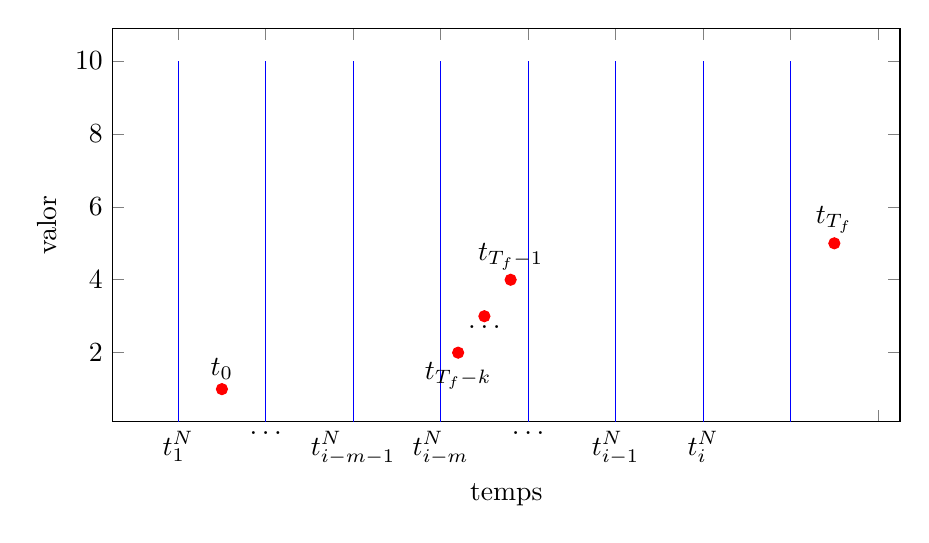
\begin{tikzpicture}
    \begin{axis}[
        width=10cm,scale only axis, height=5cm,
        xlabel=temps ,
        ylabel= valor,
        xticklabels={0,$t_1^N$,$\ldots$,$t_{i-m-1}^N$,$t_{i-m}^N$,$\ldots$,$t_{i-1}^N$,$t_i^N$},
        ]
    \addplot[ycomb,blue] coordinates {
        (0,10)
        (10,10)
        (20,10)
        (30,10)
        (40,10)
        (50,10)
        (60,10)
        (70,10)
    }; 
 
    \addplot[only marks,mark=*,red] coordinates {
        (5,1)
        (32,2)
        (35,3)
        (38,4)
        (75,5)
    };

    \node[above] at (axis cs:5,1) {$t_0$};
    \node[below] at (axis cs:32,2) {$t_{T_f -k}$};
    \node[below] at (axis cs:35,3) {$\ldots$};
    \node[above] at (axis cs:38,4) {$t_{T_f -1}$};
    \node[above] at (axis cs:75,5) {$t_{T_f}$};

    \end{axis}
  \end{tikzpicture}
  \caption{Representació d'inframostreig}
  \label{fig:rrdtool-etapes:inframostreig}
\end{figure}


Llavors per normalitzar amb inframostreig RRDtool utilitza el valor del següent interval. En aquest cas se suposa que les mesures no tenen termini, més endavant s'afegeix el problema del termini (vegeu apartat~\ref{sec:rrdtool-etapes:termini}).

És a dir, quan entre dues mesures hi ha més temps que el temps de mostreig llavors el valor de l'última mesura $\mathbf{x}(t_{T_f})$ s'expandeix enrere fins arribar a l'altra $\mathbf{x}(t_{T_f-1})$  i es calcula el valor normalitzat d'aquest gran interval. Si hi ha inframostreig però no hi ha ultramostreig
$$
t^N_{i-m-1} < t_{T_f-1} < t^N_{i-m} 
$$ 
el valor normalitzat és:
$$
x^N = \frac{ (t_{T_f-1}-t^N_{i-m-1})x_{f-1} + (t^N_i-t_{T_f-1})x_f }{t^N_i - t^N_{i-m-1}}
$$

Generalitzant, si alhora hi ha inframostreig i ultramostreig, representat a la figura~\ref{fig:rrdtool-etapes:inframostreig},
\[
t^N_{i-m-1} <  t_{T_f-k} <\cdots< t_{T_f-1}  < t^N_{i-m} 
\] 
el valor normalitzat es calcula de la mateixa manera que a l'equació~\ref{eq:rrdtool:ultramostreig}, però en l'interval $[t^N_{i-m-1},t^N_i]$:
\begin{equation}\label{eq:rrdtool:inframostreig}
x^N = \frac{ (t_{T_f-k}-t^N_{i-m-1})x_{f-k} + \cdots + (t_{T_f-1}-t_{T_f-2})x_{f-1} + (t^N_{i}-t_{T_f-1})x_f }{t^N_i - t^N_{i-m-1}}
\end{equation}

Finalment, aquest valor normalitzat per inframostreig, hi hagi ultramostreig o no, és utilitzat en tots els intervals afectats:
\[
x^N = x^N_{i-m} = \cdots = x^N_{i}
\]


Es modifica l'algoritme de càlcul iteratiu anterior segons aquest inframostreig:

\begin{lstlisting}[mathescape=true]
Normalització d'una sèrie temporal amb inframostreig
a períodes de mostreig regulars 
INPUT: 
      vector de valors $\mathbf{X} = [x_0,x_1,\ldots,x_f]$ 
      vector de temps $\mathbf{t} = [t_0,t_1,\ldots,t_f]$
      període de mostreig regular  $t_m$
OUTPUT: 
      vector de valors normalitzats $\mathbf{X^N} = [x_0^N,x_1^N,\ldots,x_k^N]$

$x_0^N$ := unknown
$t_0^N$ := 0
$t_1^N$ := $t_0^N$ + $t_m$
i := 1

$A$ := $x_0t_0$
k := 1

mentre k $\leq$ dim(x) fes
    si $t_k < t_i^N$ llavors
        $A$ := $A + x_k( t_k-t_{k-1} )$
        k := k+1
    sino 
        $N_{inf}$ := $(t_k-t_i^N)$ div $t_m$ <-- n. d'intervals amb inframostreig

        $x_i^N$ := $\dfrac{A + x_k( t_i^N-t_{k-1} ) + x_k \cdot N_{inf} \cdot t_m}{t_m  (1+N_{inf})}$

        mateix valor per cada interval amb inframostreig
        $x_{i+N_{inf}}^N$ := $\,\cdots\,$ := $x_{i+1}^N$ := $x_i^N$
        $t_{i+1}^N$ := $t_i^N + (N_{inf}+1) t_m$
        i := i + ($N_{inf}$+1)
                
        $A$ := $x_k( t_k-t_{i-1}^N )$
        k := k+1
    fsi 
fmentre
\end{lstlisting}

\paragraph{Exemple}

Agafem una nova base de dades velocitat.rrd i ara l'actualitzem amb el mateix perfil de velocitat de la figura~\ref{fig:rrdtool:mostreig_regular} però en algun interval no hi ha mostres, com es veu a la figura~\ref{fig:rrdtool:inframostreig}. És important ressaltar que aquests intervals no compleixen el període de mostreig
 Així ara el valors de velocitat mesurats són $x=[0, 0{,}5 , 2{,}5 , 3{,}8 , 2 , 0]$ en els temps $t=[10, 15, 35, 48, 55, 65]$.

\begin{figure}[htp]
  \centering
  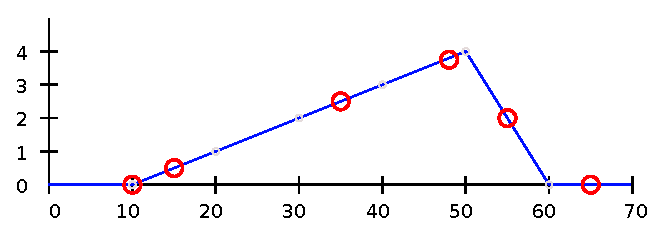
\includegraphics[width=\textwidth]{imatges/rrdtool/inframostreig.eps}
  \caption{Inframostreig: perfil de velocitat en blau, punts de mesura (alguns inframostrejats) en vermell, període de mostreig de 10 segons}
  \label{fig:rrdtool:inframostreig}
\end{figure}



S'insereixen els valors a la base de dades:
\begin{lstlisting}[style=sh]
rrdtool update velocitat.rrd 1262304010:0 1262304015:0.5 1262304035:2.5 1262304048:3.8 1262304055:2 1262304065:0
\end{lstlisting}

A continuació es mostren els valors emmagatzemats i el gràfic que genera RRDtool (figura~\ref{fig:rrdtool:velocitat_inframostrejada}):
\begin{lstlisting}
00:00:00 UTC  --> <row><v>NaN</v></row>
00:00:10 UTC  --> <row><v>0.0000000000e+00</v></row>
00:00:20 UTC  --> <row><v>2.0000000000e+00</v></row>
00:00:30 UTC  --> <row><v>2.0000000000e+00</v></row>
00:00:40 UTC  --> <row><v>3.1500000000e+00</v></row>
00:00:50 UTC  --> <row><v>3.4400000000e+00</v></row>
00:01:00 UTC  --> <row><v>1.0000000000e+00</v></row>
\end{lstlisting}


\begin{figure}[htp]
  \centering
  \includegraphics[width=\textwidth]{imatges/rrdtool/velocitat_inframostrejada.eps}
  \caption{Valors emmagatzemats a RRDtool d'un inframostreig}
  \label{fig:rrdtool:velocitat_inframostrejada}
\end{figure}


Respecte a la figura~\ref{fig:rrdtool:velocitat_irregular} del cas de mostreig en temps real, aquest gràfic només es diferencia en els intervals inframostrejats.
Ara els intervals afectats per l'inframostreig $(10,20]$ i $(20,30]$ tenen el mateix valor de 2, el qual resulta d'aplicar l'equació~\ref{eq:rrdtool:inframostreig}:  
$
x_{20}^N = x_{30}^N  = 
\frac{ (15-10) 0{,}5 + (30-15) 2{,}5 }{30 - 10}
= 2
$.
En aquests dos intervals hi ha una pitjor aproximació a la velocitat real ja que s'ha mostrejat molt poc.



\subsection{Tractament de dades desconegudes}

En les seccions anteriors, les mesures de les sèries temporals sempre tenen un valor numèric. En concret són números reals ($\mathbb{R}$), els quals es representen informàticament amb el format numèric de precisió doble seguint l'estàndard IEEE 754,~\cite{wiki:ieee754}.
 
Però les mesures, a més a més de tenir un valor, també poden ser desconegudes (\emph{unknown data}); és a dir, que no existeixin o que s'ignorin (es descartin).  Aquests valors desconeguts també estan contemplats a l'estàndard IEEE 754 i es representen  amb el valor numèric especial NaN (\emph{Not a Number}). 

L'algoritme de normalització d'intervals ha de saber manipular les mostres amb mesures desconegudes. En el cas de RRDtool, les dades desconegudes poden venir per tres vies:

\begin{itemize}
\item la mesura no existeix,
\item el temps de mesura ha superat el termini o
\item el valor de mesura està fora dels límits.
\end{itemize}

A continuació es detallen aquestes tres vies i al final es modifica l'algoritme de normalització en concordança amb el tractament d'aquestes dades desconegudes.

\subsubsection{Mesura inexistent}

Una mesura no existeix quan no s'ha pogut establir contacte amb el sensor o quan aquest retorna valors que no són númerics. Quan una mesura no existeix, es considera desconeguda i s'insereix a la base de dades amb el valor 'U' (\emph{unknown}) tot i que queda representat amb el valor NaN segons l'estàndard IEEE 754. 


Les mesures també es desconeixen quan s'inicialitza la base de dades. A l'inici d'una base de dades RRDtool es creen tots els registres fins al temps actual però aquestes mesures no han existit mai; per tant prenen 'desconegut' com a valor.


\paragraph{Exemple} S'insereix una dada amb valor conegut i l'altra amb valor desconegut

\begin{lstlisting}[style=sh]
rrdtool update velocitat.rrd 1262304010:1 1262304020:U 
\end{lstlisting}

\begin{lstlisting}
23:59:30 UTC  --> <row><v>NaN</v></row>
23:59:40 UTC  --> <row><v>NaN</v></row>
23:59:50 UTC  --> <row><v>NaN</v></row>
00:00:00 UTC  --> <row><v>NaN</v></row>
00:00:10 UTC  --> <row><v>1.0000000000e+00</v></row>
00:00:20 UTC  --> <row><v>NaN</v></row>
\end{lstlisting}

Per una banda, tots els valors anteriors al temps 0 (aquest inclòs) són desconeguts perquè no es coneix res abans que s'inicialitzi la base de dades. Per altra banda, s'ha inserit un valor numèric en el temps 10 i el valor 'desconegut' en el temps 20.



\subsubsection{Temps de termini}
\label{sec:rrdtool-etapes:termini}

El temps de termini, el qual RRDtool anomena \emph{heartbeat} ($t_h$), és el temps màxim que s'admet entre dues mesures. La mesura actual s'ignora si ha passat més temps que el termini des de la mesura anterior. 
$$
t_i - t_{i-1} > t_h \longrightarrow   x(t_i) = unknown 
$$
 
A RRDtool el termini pot ser més gran, igual o més petit que el temps de mostreig. És a dir, que el termini no només afecta en els casos d'inframosteig sinó que també al casos d'ultramostreig.


Cal no confondre el termini de RRDtool (\emph{heartbeat})  amb el termini utilitzat pels sistems de temps real (\emph{deadline}). El \emph{heartbeat} es mesura entre mostres amb l'objectiu de tenir dades 'fresques' i en canvi el \emph{deadline} es mesura a partir del temps d'activació amb l'objectiu de complir temps de càlcul. En el cas de tasques periòdiques, com és el cas del temps de mostreig a RRDtool, en temps real no té sentit parlar de terminis més grans que el període de mostreig, en canvi en els RRDtool ja s'ha vist que poden tractar aquestes situacions, anomenades inframostreig.


A continuació s'estudien  quatre casos diferents segons els valors que pot adoptar el temps de termini respecte del temps de mostreig. Els quatre casos es poden veure a l'eix vertical de la figura~\ref{fig:rrdtool:terminis} representant el termini amb $t_h$, el període de mostreig amb $t_m$ i exemples de temps de mesura amb una circumferència vermella a l'eix horitzontal. 

\begin{figure}[htp]
  \centering
  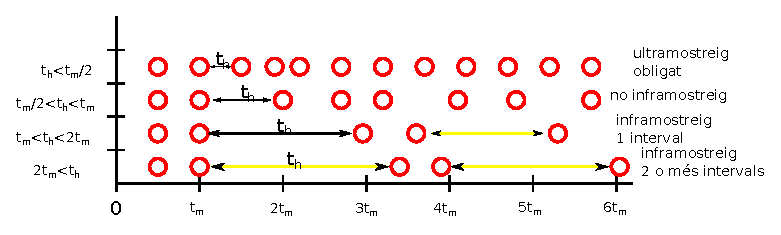
\includegraphics[width=\textwidth]{imatges/rrdtool/terminis.eps}
  \caption{Comparació de mostrejos amb terminis $t_h$ diferents pel mateix període de mostreig $t_m$, punts de mesura en vermell i intervals inframostrejats en groc}
  \label{fig:rrdtool:terminis}
\end{figure}

Primer de tot, del concepte de RRDtool es desprèn que en qualsevol cas sempre hi pot haver ultramostreig. Això és degut a que els terminis són els temps màxims entre mesures però no s'especifica un temps mínim. Aquestes situacions es poden veure a la figura~\ref{fig:rrdtool:terminis}: a l'eix horitzontal hi ha marcats els temps de mostreig exactes però el temps de mesura pot prendre qualsevol valor mentre sigui inferior al termini prefixat.


Un termini més gran que el temps de mostreig  ($t_h>t_m$) indica que s'accepten els casos d'inframostreig i el temps del termini limita el temps durant el qual es permet no disposar de mesures. A més, si el termini és més petit que el doble del temps de mostreig ($t_m<t_h<2t_m$), com a màxim només hi pot haver un interval amb inframostreig. Però si el termini supera el doble del temps de mostreig, llavors l'inframostreig es pot donar en dos intervals, en tres intervals si és el triple, etc.

Un termini més petit que el temps de mostreig ($t_h<t_m$) indica que no es vol inframostreig; és a dir que en cada interval com a mínim hi ha d'haver una mostra. Però, al mateix temps, un termini més petit que el temps de mostreig fa que a la llarga s'obligui a ultramostrejos en alguns intervals. Encara més, si el termini és inferior a la meitat del temps de mostreig, llavors hi ha d'haver ultramostreig en tots els intervals.

Normalment, en els usos de RRDtool, el valor del termini s'assigna a un valor més gran que el doble del temps de mostreig ($t_h>2t_m$) per tal de poder tenir folgança en les mesures. Cal observar que el cas del mostreig únic es representa amb el termini doblant el temps de mostreig ($t_h=2t_m$); això permet que la mesura següent se situi en qualsevol temps de l'interval de mostreig següent.

El cas del mostreig únic és comparable als sistemes en temps real. En els sistemes en temps real el temps entre mostres com a màxim pot doblar el temps de mostreig, mentre es compleixi que en cada interval de mostreig hi ha una mostra. En el cas de RRDtool, quan $t_h=2t_m$, hi pot haver inframostreig i per tant es pot no complir el temps real requerit pel mostreig únic. 
En conclusió, el temps de termini a RRDtool només s'utilitza per avaluar si les dades són 'fresques', la responsabilitat de les mesures i del temps real recau a la part d'adquisició de dades dels sistemes de monitoratge. 

A RRD el termini es defineix a l'hora de crear una base de dades però es pot tornar a configurar. Cada variable mesurada (cada registre) té el seu termini.


\paragraph{Exemple} Ara es crea la base de dades velocitat.rrd amb un temps de mostreig de 10 segons i un termini de 6 segons.

\begin{lstlisting}[style=sh]
rrdtool create velocitat.rrd --start 1262304000 --step 10 \
        DS:mps:GAUGE:6:-U:U                             \
        RRA:AVERAGE:0.5:1:24                                 
\end{lstlisting}

S'actualitza la base de dades amb els valors $x=[1,1,1]$ en els temps $t=[6,10,20]$.

\begin{lstlisting}[style=sh]
rrdtool update velocitat.rrd 1262304006:1 1262304010:1 1262304020:1 
\end{lstlisting}

A continuació es mostren els valors emmagatzemats:
\begin{lstlisting}
00:00:00 UTC  --> <row><v>NaN</v></row>
00:00:10 UTC  --> <row><v>1.0000000000e+00</v></row>
00:00:20 UTC  --> <row><v>NaN</v></row>
\end{lstlisting}

Les mesures implicades en el primer interval [0,10] han complert els terminis ja que el temps entre mesures és igual o inferior a 6 segons. Però en el segon interval [10,20], l'última mesura dista 10 segons respecte de l'anterior i per tant s'ignora i es considera desconeguda. 


\subsubsection{Límits}

Una altra comprovació que es fa a les mesures és si estan dins d'un rang. A RRDtool es comprova que el valor mesurat és més gran que un límit inferior i que és més petit que un límit superior. Si la mesura està fora de rang, s'ignora i es considera desconeguda.
$$
x(t_i) > L_{\max}  \longrightarrow   x(t_i) = unknown 
$$
$$
x(t_i) < L_{\min} \longrightarrow   x(t_i) = unknown 
$$

El límits sempre es calculen a les mesures un cop ja han passat l'etapa de transformació a velocitat. En el cas dels comptadors es comprova que la velocitat calculada estigui dins del rang però no es comprova la magnitud comptada, és a dir el valor que realment s'ha mesurat.

A RRDtool els límits es defineixen a l'hora de crear una base de dades però es poden tornar a configurar. Cada variable mesurada, això és cada registre, té el seus límits. Si no es vol comprovar el rang de les mesures, els límits es poden configurar amb el valor desconegut (\emph{U}) per tal que no es tinguin en compte. 


\paragraph{Exemple} Ara es crea la base de dades velocitat.rrd amb un límit inferior de 0 i un límit superior desconegut.

\begin{lstlisting}[style=sh]
rrdtool create velocitat.rrd --start 1262304000 --step 10 \
        DS:mps:GAUGE:600:0:U                             \
        RRA:AVERAGE:0.5:1:24                                 
\end{lstlisting}

Ara s'actualitza la base de dades amb els valors $x=[0,1000,-1]$ en els temps $t=[10,20,30]$.

\begin{lstlisting}[style=sh]
rrdtool update velocitat.rrd 1262304006:1 1262304010:1 1262304020:1 
\end{lstlisting}

A continuació es mostren els valors emmagatzemats:
\begin{lstlisting}
00:00:00 UTC  --> <row><v>NaN</v></row>
00:00:10 UTC  --> <row><v>0.0000000000e+00</v></row>
00:00:20 UTC  --> <row><v>1.0000000000e+03</v></row>
00:00:30 UTC  --> <row><v>NaN</v></row>
\end{lstlisting}

No hi ha límit superior però sí que n'hi ha d'inferior. En el temps 30 el valor és més petit que el límit i per tant s'ignora la mesura i es considera desconeguda.


\subsubsection{Càlcul amb dades desconegudes}

Fins ara s'ha vist les tres vies per on es poden obtenir dades desconegudes en la normalització d'intervals. Cal notar que les tres vies només serveixen per considerar si una mesura és desconeguda o no, però una mesura desconeguda no és suficient per considerar tot l'interval normalitzat desconegut.

A RRDtool, l'interval es considera desconegut\footnote{A l'etapa de normalització d'interval no es pot triar la quantitat de desconeguts que són acceptables, ni fins i tot poder decidir si un valor desconegut ja fa calcular tot l'interval com desconegut. A l'etapa de consolidació sí que és possible (v.\ secció~\ref{rrdtool:consolidacio:unknown}).}
quan el temps de mesures desconegudes ($T_u$)  és superior a la meitat del període de mostreig.
$$
T_u = \sum_{\forall x_f = unknown} ( t_f-t_{f-1} ) \quad
$$
$$
\text{si } T_u > t_m/2  \longrightarrow   x^N_{t^N_i} = unknown 
$$
sent $T_u$ el temps total que en un interval els valors $\mathbf{X}$ prenen valor desconegut.

En cas contrari es calcula l'interval amb els valors coneguts. És a dir, l'algoritme de normalització d'intervals ha de saber manipular les mostres amb mesures desconegudes. 
Per normalitzar, les dades desconegudes es considera que valen la mitjana de l'interval ($x_i^N=x_u$) .  D'aquesta manera no afecta a la velocitat mitjana de l'interval. Tot seguit es demostra.

\begin{figure}[tbp]
  \centering
  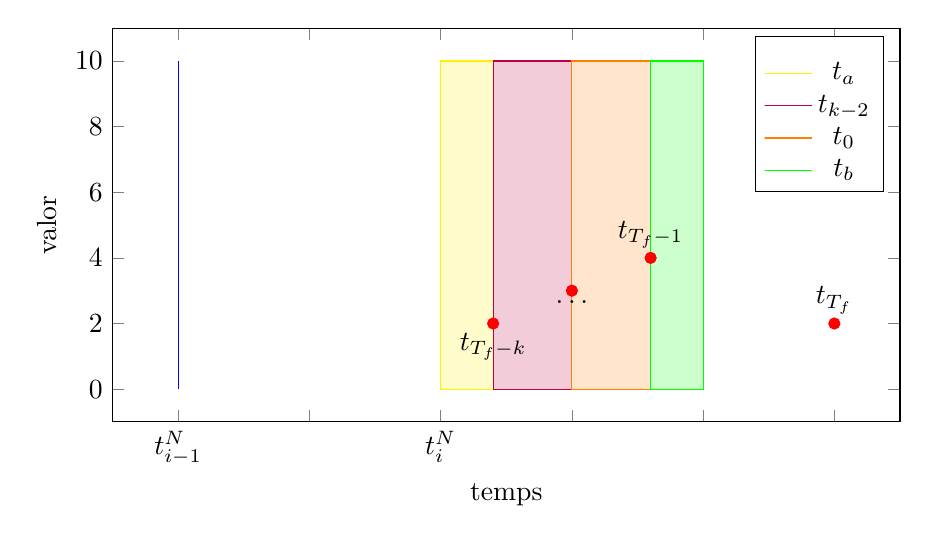
\begin{tikzpicture}
    \begin{axis}[
        width=10cm,scale only axis, height=5cm,
        xlabel=temps ,
        ylabel= valor,
        xticklabels={$\ldots$,,$t_{i-1}^N$,,$t_i^N$},
        ]
    \addplot[ycomb,blue] coordinates {
        (20,10)
        (30,10)
        (40,10)
    }; 
    \addlegendentry{}

    \addplot[ybar interval,yellow,fill=yellow!20!white] coordinates{
        (30,0)
        (30,10)
        (32,10)
        (32,0)
    };
    \addlegendentry{$t_a$}

   \addplot[ybar interval,purple,fill=purple!20!white] coordinates{
        (32,0)
        (32,10)
        (35,10)
        (35,0)
    };
    \addlegendentry{$t_{k-2}$}

    \addplot[ybar interval,orange,fill=orange!20!white] coordinates{
        (35,0)
        (35,10)
        (38,10)
        (38,0)
    };
    \addlegendentry{$t_0$}

    \addplot[ybar interval,green,fill=green!20!white] coordinates{
        (38,0)
        (38,10)
        (40,10)
        (40,0)
    };
    \addlegendentry{$t_b$}
 

 
    \addplot[only marks,mark=*,red] coordinates {
        (32,2)
        (35,3)
        (38,4)
        (45,2)
    };

    \node[below] at (axis cs:32,2) {$t_{T_f -k}$};
    \node[below] at (axis cs:35,3) {$\ldots$};
    \node[above] at (axis cs:38,4) {$t_{T_f -1}$};
    \node[above] at (axis cs:45,2) {$t_{T_f}$};



    \end{axis}
  \end{tikzpicture}
  \caption{Representació d'ultramostreig simplificada}
  \label{fig:rrdtool-etapes:desconeguts}
\end{figure}


Per una banda, la mitjana de l'interval sense tenir en compte els valors desconeguts es calcula utilitzant l'equació~\eqref{eq:rrdtool:ultramostreig} només en els valors coneguts. Per facilitar la comprensió, es reescriu l'equació utilitzant $t_a$, $t_b$ i $t_j$, representats a la figura~\ref{fig:rrdtool-etapes:desconeguts}:
$$%
t_a =t_{T_f-k}-t^N_{i-1} \quad\text{ i }\quad t_b = t^N_i-t_{T_f-1}
$$
$$
t_j =t_{T_f-1-j}-t_{T_f-2-j} \quad\forall j=[0,k-2]
$$
\begin{equation}\label{eq:rrdtool:normalitzacio}
x^N_i = \frac{t_ax_a+\sum\limits_{j=0}^{k-2} (t_jx_j)+t_bx_b}{t_a+\sum\limits_{j=0}^{k-2} (t_j)+t_b}
\end{equation}
Per altra banda, l'equació tenint en compte els valors desconeguts ($x_u$) és
\begin{equation}\label{eq:rrdtool:normalitzacio-desconegut}
x^N_i = \frac{t_ax_a+\sum\limits_0^{k-2} (t_jx_j)+t_bx_b+T_ux_u}{t_a+\sum\limits_0^{k-2} (t_j)+t_b+T_u}
\end{equation}
Substituint \eqref{eq:rrdtool:normalitzacio} a \eqref{eq:rrdtool:normalitzacio-desconegut} 
\[
x^N_i = \frac{ x_i^N(t_a+\sum\limits_0^{k-2} (t_j)+t_b)+T_ux_u}{t_a+\sum\limits_0^{k-2} (t_j)+t_b+T_u}
\]
operant amb aquesta expressió
\begin{align*}
 x^N_i - \frac{ x_i^N(t_a+\sum\limits_0^{k-2} (t_j)+t_b)+T_ux_u}{t_a+\sum\limits_0^{k-2} (t_j)+t_b+T_u} &= 0\\
 \frac{x^N_i(t_a+\sum\limits_0^{k-2} (t_j)+t_b+T_u) -  x_i^N(t_a+\sum\limits_0^{k-2} (t_j)+t_b)-T_ux_u}{t_a+\sum\limits_0^{k-2} (t_j)+t_b+T_u} &= 0\\
\frac{T_ux_i^N+T_ux_u}{t_a+\sum\limits_0^{k-2} (t_j)-t_b+T_u} &= 0
\end{align*}
Aleshores
\[
x_i^N = x_u
\]


Per tant si els valors desconeguts valen el mateix que la mitjana ($x_u=x^N_i$), aquesta mitjana es pot calcular senser tenir-los en compte com a l'equació~\ref{eq:rrdtool:normalitzacio}. En aquesta equació el temps de l'interval queda reduït, ja que el temps total de l'interval equival al temps de mostreig
$$
t_m= t_a+\sum\limits_0^{k-2} (t_j)+t_b+T_u
$$
i per tant es pot reexpressar a l'eq.~\ref{eq:rrdtool:normalitzacio} com el temps de mostreig descomptant-hi els temps en valors desconeguts
$$
t_a+\sum\limits_0^{k-2} (t_j)+t_b = t_m -T_u
$$

En resum, la normalització de l'interval es pot calcular amb l'àrea acumulada dels valors sense comptar-hi els desconeguts i al final dividida entre el temps de mostreig descomptant-hi els temps en valors desconeguts
$$
x^N_i = \frac{t_ax_a+\sum\limits_0^{k-2} (t_jx_j)+t_bx_b}{t_m - T_u}
\quad\forall\ x(t)\neq unknown
$$


Com que es dóna un valor al desconegut, això fa que la magnitud comptada augmenti. És a dir, s'està suposant que el comptador ha seguit mesurant a una velocitat semblant a les altres de l'interval.

Aquest augment s'observa seguint l'equació $e=x(t)$
$$
e_{mesurat} = x_at_a+\sum\limits_0^{k-2} (x_jt_j)+x_bt_b
$$
$$
e_{emmagatzemat} = x_at_a+\sum\limits_0^{k-2} (x_jt_j)+x_bt_b+x^N_iT_u
$$



% Atenció: sembla que hi ha un bug

% Heartbeat=600. Mentre que 
% rrdtool updatev consolida.rrd 1262304015:1 1262304030:U dóna 1(?),1(no) updatev consolida.rrd 1262304015:1 1262304029:U 1262304030:U dóna 1(bé),U(bé)

% però si Heartbeat=12 dóna U,U


% Un altre bug. Heartbeat=3 rrdtool updatev consolida.rrd 1262304013:1 1262304016:1 1262304019:1 1262304022:1 dóna 1(bé). rrdtool updatev consolida.rrd 1262304013:1 1262304017:1 1262304020:1 dóna 1(bé). però rdtool updatev consolida.rrd 1262304013:1 1262304016:1 1262304020:1 dóna U(no)

% %http://www.vandenbogaerdt.nl/rrdtool/total.php
% %http://www.mrtg.org/rrdtool/doc/rrdcreate.en.html



\subsection{Algoritme de normalització}
Ara es modifica l'algoritme tenint compte les dades desconegudes i també els ultramostrejos i inframostrejos dels intervals. Aquest és l'algoritme complet de normalització d'intervals.



\begin{lstlisting}[mathescape=true]
Normalització d'una sèrie temporal
a períodes de mostreig regulars 
INPUT: 
      vector de valors $\mathbf{X} = [x_0,x_1,\ldots,x_f]$ 
      vector de temps $\mathbf{T} = [t_0,t_1,\ldots,t_f]$
      període de mostreig regular  $t_m$
      termini $H$
      llindars màxim $X^{MAX}$ i mínim $X^{MIN}$
OUTPUT: 
      vector de valors normalitzats $\mathbf{X^N} = [x_0^N,x_1^N,\ldots,x_k^N]$

$x_0^N$ := unknown <-- primer valor normalitzat desconegut
$t^N$ := $t_m$ <-- següent interval de normalització
i := 1

$A$ := 0 <--- àrea acumulada
$t_{ant}$ := 0 <-- temps de la mostra anterior
$T_u$ := 0 <-- temps en valor desconegut

per cada parella $(x,t)$ en $\mathbf{X}$ i $\mathbf{T}$ fes:

    avalua termini i llindar:
    si $t-t_{ant}$ > $H$ o no $X^{MIN}$ $\leq$ x $\leq$ $X^{MAX}$ llavors x:= unknown fsi

    si $t < t^N$ llavors
        si x = unknown llavors
            $T_u$ := $T_u + t -t_{ant}$ <-- acumula temps desconegut
        sino
            $A$ := $A + x( t-t_{ant} )$ <-- acumula valor
        fsi

    sino  <-- càlcul d'un valor normalitzat

        $N_{inf}$ := $(t-t^N)$ div $t_m$ <-- n. d'intervals amb inframostreig

        si x = unknown llavors
            $T_u$ := $T_u+t^N -t_{ant} +N_{inf}\cdot t_m$ <-- acumula temps desconegut
        sino
            $x_i^N$ := $A + x( t^N-t_{ant} ) + x \cdot N_{inf} \cdot t_m$ <-- acumula valor
        fsi

        si $T_u > \frac{(1+N_{inf})t_m}{2}$ llavors
            $x_i^N$ := unknown <--  normalitza desconegut
        sino
            $x_i^N$ := $\dfrac{A}{t_m (1+N_{inf})-T_u}$ <--  normalitza valor
        fsi

        mateix valor per cada interval amb inframostreig
        $x_{i+N_{inf}}^N$ := $\,\cdots\,$ := $x_{i+1}^N$ := $x_i^N$
                
        si x = unknown llavors <-- acumula desconegut, reset àrea 
            $T_u$ := $t-t_{ant}$
            $A$ := 0
        sino <-- acumula àrea, reset desconeguts
            $T_u$ := 0
            $A$ := $x( t-t^N )$
        fsi

        $t^N$ := $t^N + (N_{inf}+1) t_m$ <-- següent interval de normalització
        i := i + ($N_{inf}$+1)

    fsi 

    $t_{ant}$ := $t$

repeteix
\end{lstlisting}




\section[Consolidació]{Consolidació d'intervals}

Un cop s'ha normalitzat l'interval, a la base de dades hi ha els valors amb temps de mostreig regular (\emph{step}). Aquest valors ja normalitzats a RRDtool s'anomenen \emph{Primary Data Points} (PDP). 

Però aquest interval de mostreig inicial no es pot mantenir durant gaire temps ja que cada cop és més difícil gestionar la quantitat de dades. Per afitar la quantitat de dades emmagatzemades, RRDtool desa les dades en diferents resolucions temporals. 

És a dir, cal consolidar l'interval normalitzat inicial a altres temps de mostreig desitjats. A partir dels PDP es tornen a mostrejar (\emph{resampling}) nous intervals amb menys resolució. 

A RRDtool, aquest valors nous consolidats s'anomenen \emph{Consolidated Data Points} (CDP) i cada resolució s'emmagatzema en les taules anomenades \emph{Round Robin Archive} (RRA).
Cada CDP es calcula a partir de $n$ PDP i cada RRA defineix aquest $n$ necessari, el qual a RRDtool s'anomena \emph{step} però que cal no confondre'l amb l'\emph{step} de normalització d'interval. Es poden distingir com a \emph{step de CDP} i \emph{step de PDP}, respectivament.


En aquest càlcul pot interessar conservar diferent informació de les variables mesurades. El canvi de resolució implica una pèrdua de precisió i informació, cal trobar un càlcul que mantingui les propietats que interessin de les dades

Per un RRA que aplica una funció $f$ de consolidació a $n$ PDP (valors normalitzats $V^N$) per obtenir un CDP:
$$
CDP_i = f(x^N_{i-n},\ldots,x^N_i) \qquad i \in \{ n,2n,3n\ldots \}
$$

És a dir que la resolució dels CDP sempre és múltiple del temps de mostreig base dels PDP. 
Actualment RRDTool permet calcular quatre funcions de consolidació: 

\begin{itemize}
\item mitjana (AVERAGE)
\item màxim (MAX)
\item mínim (MIN)
\item últim (LAST)
\end{itemize}

% Aquestes funcions tenen la particularitat que es poden calcular de manera incremental.
% $$
% CDP_i =   f(f( \ldots( f(f(unknown,x^N_{i-n}), x^N_{i-n+1}),\ldots ), x^N_{i-1}) ,x^N_i )  \qquad i \in \{ n,2n,3n\ldots \}
% $$


Calcular la mitjana és equivalent al que es fa a l'etapa de normalització de l'interval. En aquell cas cal fer una mitjana ponderada per la durada de la mesura però ara els intervals són iguals per tots els valors i per tant ja no cal considerar el temps. 
$$
\text{CDP}_i(\text{AVERAGE}) = \frac{\sum\limits_{k=1}^N t_m\text{PDP}_k }{\sum\limits_{k=1}^N t_m}
= \frac{t_m\sum\limits_{k=1}^N \text{PDP}_k}{nt_m}
= \frac{\sum\limits_{k=1}^N \text{PDP}_k}{n}
$$
on $n$ és el total de valors normaitzats que s'agafen, el qual s'ha anomenat \emph{step de CDP}.

Per als càlculs de màxim, mínim i últim cal recordar que s'apliquen als PDP, és a dir un cop els valors mesurats han estat normalitzats. Per exemple en el cas del màxim no es conserva el valor més alt que s'ha mesurat sinó el valor més alt dels PDP; un cop s'ha fet la mitjana ponderada de les mesures. 

Una altra lectura possible és que en un RRA que calculi cada CDP amb un PDP tant és quina funció s'apliqui; els CDP seran iguals als PDP.

\subsection{Dades deconegudes}\label{rrdtool:consolidacio:unknown}

A la sortida de l'etapa de normalització, alguns intervals poden prendre el valor 'desconegut' (\emph{unknown}). Les funcions de consolidació han de calcular amb aquests valors i per tant han de decidir com tractar-los.

Per una banda, quan l'etapa de normalització es troba valors desconeguts en un interval de mostreig, aproximació la normalització de manera que els valors desconeguts no alterin la mitjana dels valors coneguts. 
Ara a l'etapa de consolidació també s'aplica el mateix criteri per a la funció de consolidació de mitjana: com s'ha fet per $x_u=x_i^N$ a  \eqref{eq:rrdtool:normalitzacio} a \eqref{eq:rrdtool:normalitzacio-desconegut} ara s'aplica el mateix a $x_U=\text{CDP}_i$ i aleshores es pot escriure
$$
\text{CDP}_i(\text{AVERAGE}) = \frac{\sum\limits_{k=1}^N \text{PDP}_k}{n_{\text{coneguts}}} = \frac{x_u+\sum\limits_{k=1}^N \text{PDP}_k }{n}
$$


Però hi ha altres funcions i cal generalitzar el criteri. Per a les funcions de mínim i màxim es considera que els valors desconeguts no afecten en el càlcul i per a la funció d'últim el valor consolidat pren el que calgui, valor o 'desconegut'. Per tant, aquestes funcions no es veuen afectades per $n$.

Per altra banda, a l'etapa de normalització es considera un interval desconegut quan més de la meitat de l'interval de mostreig té valors desconeguts. 
Però ara, a l'etapa de consolidació, hi ha un paràmetre que permet decidir el percentatge de valors desconeguts que calen perquè el valor consolidat sigui considerat desconegut. Aquest paràmetre s'anomena xff (\emph{xfiles factor}\footnote{RRDtool l'anomena el factor d'expedients X (\emph{X-Files Factor}) perquè si té un valor diferent de zero el resultat està fora dels límits científics,~\cite{vandenbogaerdt}}).
$$
N_{\text{desconeguts}}/N > \text{xff} \longrightarrow \text{CDP}_i = unknown
$$
on l'xff s'expressa en tant per u. 

A continuació es resumeix el tractament de desconeguts en un algoritme
\begin{lstlisting}[mathescape=true]
Consolidació d'una sèrie temporal
cada període de consolidació segons els valors normalitzats
INPUT: 
      vector de valors normalitzats $\mathbf{PDP} = \mathbf{X^N} = [x_0^N,x_1^N,\ldots,x_k^N]$
      funció d'interpolació $f$
      període de consolidació  $N$ en n. de PDP
      llindar de desconeguts $x^{ff}$ en tant per u
OUTPUT: 
      vector de valors consolidats $\mathbf{CDP} = [cdp_0,cdp_1,\ldots,cdp_l]$

i := 0
$cdp_i$ := unknown

$a$ := 0 <-- acumulador pels interpoladors
$T_u$ := 0 <-- Temps en valor desconegut
$n$ := 1 <-- quantitat de PDP calculats

per cada $p$ a $\mathbf{PDP}$ fes:

    si $p$ = unknow llavors
        $T_U$ := $T_u + 1$ <-- acumula temps desconegut
    
    sino <-- aplica l'interpolador corresponent
        cas f és
            AVERAGE $\longrightarrow$ $a$ := $\dfrac{a(n-1) + p}{n}$  
            MAX $\longrightarrow$ $a$ := $\max(a, p)$  
            MIN $\longrightarrow$ $a$ := $\min(a, p)$  
            LAST $\longrightarrow$ $a$ := $p$  
        fcas
    fsi

    si $n = N$ llavors <-- consolida

        si $T_u$ / N > $x^{ff}$ llavors
            $cdp_i$ := unknown <-- consolida desconegut
        sino
            $cdp_i$ ::= acumulat <-- consolida el valor
        fsi
        i := i+1 
        $n$ := 0
        $a$ := 0
        $T_u$ := 0
    fsi
    n := n + 1
repeteix
\end{lstlisting}






%%% Local Variables:
%%% TeX-master: "memoria"
%%% End:

% LocalWords:  RRDtool RRD Gauge width rrd UTC row NaN Counter Absolute
